\documentclass[main]{subfiles} 

\begin{document}

\chapter{IMPLEMENTATION AND CODING}
\section{Implementation}

The game is built with Object Oriented approach and SFML framework provides the underlying foundation. Box2D library is used for physics simulation with SFML. State machine or simply \texttt{State} class is the backbone of the game on top of which all the game elements are built. \texttt{State} in simple words represents the various stages of the game. All the states such as \texttt{Splash Screen State}, \texttt{Menu State}, \texttt{Game State}, etc. are derived from the \texttt{State} class.

There is \texttt{Game} class as well that handles all the types of data that need to be used across different states. It also initiates input handling, data updating and state changing mechanisms among others.

The namespace \texttt{HeadBall} wraps all the structures, classes and their members.


\subsection{States}
As aforementioned, states are the backbone of the game. The whole game is constructed upon the concept of states. When an event is taking place in the game, there is a state making that event happen. When that event is to be suspended for some time, another  state reference is pushed onto the stack and when the operation of the event is to be resumed, the corresponding state reference is brought to the top of the stack. The class handling all the stack related operations is the \texttt{StateMachine} class.

The \texttt{State} class hierarchy showing only the derived class names is given in fig. \ref{fig:state_hierarchy_classes}.

\begin{figure}[H]
  \centering
  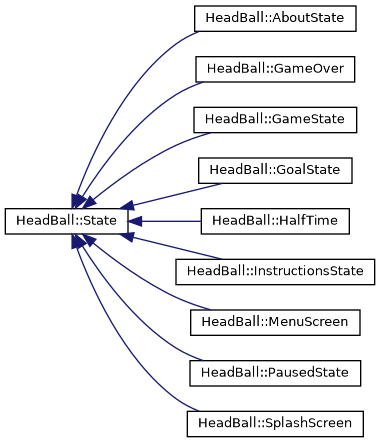
\includegraphics[scale=0.5]{graphics/UML_diagrams/state_hierarchy_brief}
  \caption{State class hierarchy with derived class names}
  \label{fig:state_hierarchy_classes}
\end{figure}

Brief descriptions of each of the derived classes of the base class \texttt{State} are given below with nestings as necessary, and are arranged in the order their occurrence from the time the game is run:

\begin{itemize}
    \item SplashScreen State:
        For the screen to show immediately before the menu screen is shown.
    
    \item MenuScreen State:
        To show menu screen having various menu options.
    
    \item Game State:
        The major state where the gameplay happens.
        \begin{itemize}
            \item Goal State:
                To show the screen when a player scores.
                
            \item Halftime State:
                To show the screen when it is halftime.
            
            \item Paused State:
                To show the screen when the game is paused.
        \end{itemize}
    
    \item GameOver State:
        To show the screen when it is fulltime or the end of the game.
        
    \item Instructions State: 
        For showing the instructions page.
    
    \item About State:
        For showing the about page.
    
\end{itemize}\


\subsection{Resource Managers}
Like there are different states to manage various stages of the game, there are a few manager classes that are used for the purpose of efficiently managing the resources and elements. These include:
\begin{itemize}
    \item AssetManager class: 
        Class for managing assets.
 
    \item InputManager class: 
        Class for handling the user inputs through mouse and keyboard.
    
    \item TimeManager class: 
        Class for handling time during games.
\end{itemize}


\section{Coding} 

%state machine: pushing popping
%loading assets and splash screen animation 
%input management:sprite clicking

%shared pointer use
%unique pointer use
%movement and kicking
%goal detection
%time management

Here are the explanations of some of the important parts of the project:

\subsection{State Management}
State management is done by the \texttt{StateMachine} class. First of all a \texttt{unique\_ptr} is defined which points to the different game states. This is made possible by inheriting all the game state classes to a common abstract class \texttt{State}. 
The inheritance diagram for this class is given in fig. \ref{fig:state_hierarchy_full}. 

The \texttt{StateMachine} class contains a stack where the different game states are kept. In every game loop, the state that is at the top of the stack gets resumed. At every game loop, the \texttt{processStateChanges} method of the \texttt{StateManager} class is called, which manages the transition from one state to another.

\begin{minted}[breaklines, bgcolor=lightgray]{cpp}
    void StateManager::processStateChanges {
        if (_isRemoving == true && !_states.empty() ) {
            this->_states.pop( );

            if (!_states.empty ( )) {
                this->_states.top( )->resume( );
            }

            this->_isRemoving = false;
        }

        if (_isAdding == true) {
            if (_isReplacing == true && !_states.empty()) {
                this->_states.pop( );
            } else if (!_states.empty()) {
                this->_states.top( )->pause( );
            }

            this->_states.push(std::move(this->_newState));
            this->_states.top( )->init( );

            this->_isAdding = false;
        }
    }
\end{minted}


Here, the bool attributes \texttt{\_isAdding}, \texttt{\_isRemoving} and \texttt{\_isReplacing} indicate whether a new state is being added, removed or replaced from the stack. These values are changed during the course of the game loop according to the input given by the user.
\begin{itemize}
    \item When a state is being removed, first of all it is checked if the stack is empty. If the stack is not empty, it pops the state that is at the top of the stack. Again it checks whether a state is empty. If it is not empty, it resumes the state that is at the top of the stack.
    \item When a state is being added, first of all it is checked whether it is being replaced or not. If it is being replaced and the stack is not empty, the top state at the stack is popped. And if it is not being popped and the stack is not empty, the top state in the stack is paused. Now, the new state is being pushed in the stack and initiated. 
\end{itemize}


\subsection{Input Management}
Input management is done by \texttt{InputManager} class.In this class, inputs given by the user is checked and a boolean value is returned which then is processed through \texttt{Game} class to provide required state output.

\begin{minted}[bgcolor=lightgray, breaklines]{cpp}
 bool InputManager::isSpriteClicked (sf::Sprite sprite, sf::Mouse::Button button, sf::RenderWindow& window) {
    if (sf::Mouse::isButtonPressed(button)) {
        sf::IntRect spriteRect (sprite.getPosition().x - sprite.getGlobalBounds().width / 2, sprite.getPosition().y - sprite.getGlobalBounds().height / 2, sprite.getGlobalBounds().width, sprite.getGlobalBounds().height); 
        if (spriteRect.contains(sf::Mouse::getPosition(window))) {
            return true;
        }
    }
    return false;
}

sf::Vector2i InputManager::getMousePosition (sf::RenderWindow& window) {
    return sf::Mouse::getPosition(window);
}

bool InputManager::isMoving (std::string position, std::string player) {
    bool isp2 = false;
    if (player == "p2") {
        isp2 = true; 
    }

    if (!isp2 && position == "left") {
        if (sf::Keyboard::isKeyPressed (sf::Keyboard::Key::P1_LEFT)) {
            return true;
        }
    }

    else if (!isp2 && position == "right") {
        if (sf::Keyboard::isKeyPressed (sf::Keyboard::Key::P1_RIGHT)) {
            return true;
        }
    }

    else if (isp2 && position == "left") {
        if (sf::Keyboard::isKeyPressed (sf::Keyboard::Key::P2_LEFT)) {
            return true;
        }
    }


    else if (isp2 && position == "right") {
        if (sf::Keyboard::isKeyPressed (sf::Keyboard::Key::P2_RIGHT)) {
            return true;
        }
    }
    return false;
}

bool InputManager::isDoing (std::string action, std::string player) {
    bool isp2 = false;
    if (player == "p2") {
        isp2 = true; 
    }

    if (!isp2 && action == "jump") {
        if (sf::Keyboard::isKeyPressed (sf::Keyboard::Key::P1_JUMP)) {
            return true;
        }
    }

    else if (!isp2 && action == "kick") {
        if (sf::Keyboard::isKeyPressed (sf::Keyboard::Key::P1_KICK)) {
            return true;
        }
    }

    else if (isp2 && action == "jump") {
        if (sf::Keyboard::isKeyPressed (sf::Keyboard::Key::P2_JUMP)) {
            return true;
        }
    }

    else if (isp2 && action == "kick") {
        if (sf::Keyboard::isKeyPressed (sf::Keyboard::Key::P2_KICK)) {
            return true;
        }
    }
    return false;
}
\end{minted}

There are four member functions of this class for four different input methods.They are:
\begin{itemize}
    \item\texttt{isSpriteClicked()} is used to check if the player has clicked the sprites or not and returns boolean value as per the input.In this function, firstly it checks whether the mouse button is pressed or not, if the button is pressed then it checks whether the sprite provided in the parameter contains the cursor and if it does then the \texttt{true} value is returned. If any of the condition is not fullfilled \texttt{false} value is returned.
    \item\texttt{getMousePosition()} is used to return the vector position of the mouse cursor in the rendering window.
    \item\texttt{isMoving()} checks if any of the player(P1,P2) is pressing the defined key to move the player and returns the boolean value.
    \item\texttt{isDoing()} checks if the player is pressing the defined key to jump or kick the ball and returns the boolean value.
\end{itemize}


\subsection{Movement of Player and Kicking Ball}
\subsubsection{Movement of Player}
\begin{minted}[bgcolor=lightgray,breaklines]{cpp}
void Player::moveLeft ( ) {
    b2Vec2 currentVelocity = this->_body->GetLinearVelocity ( );
    this->_body->SetLinearVelocity (b2Vec2(- MOVEMENT_VELOCITY , currentVelocity.y));
}
     
void Player::moveRight(){
    b2Vec2 currentVelocity = this->_body->GetLinearVelocity ( );
    this->_body->SetLinearVelocity(b2Vec2(MOVEMENT_VELOCITY, currentVelocity.y));
}
    
void Player::jump ( ) {
    b2Vec2 currentVelocity = this->_body->GetLinearVelocity ( );
    this->_body->SetLinearVelocity (b2Vec2 (currentVelocity.x, - MOVEMENT_VELOCITY));
}
\end{minted}
There are primarily three types of player movement i.e moving left, moving right and jumping. These movement is performed by calling above functions after input is provided by the user. 

Here \texttt{b2Vec2} is used to define vector in box2d world. It takes two float values as parameters. e.g A new vector can be defined as \texttt{b2Vec2 newVector(3.2f, 0.65f);} 

\texttt{GetLinearVelocity()} is a function that returns the current linear velocity of the center of mass of the body in box2d world. Syntax for this function is \texttt{const b2Vec2 \& b2Body::GetLinearVelocity( ) const}. 

Similarly \texttt{SetLinearVelocity()} sets the linear velocity to center of mass of the body in box2d world. Syntax for this function is \texttt{void b2Body::SetLinearVelocity(const b2Vec2 \&v)}

The variable \texttt{MOVEMENT\_VELOCITY} is defined in Definition.hpp header file and its value is 5.0f.

\subsubsection{Kicking Ball}
\begin{minted}[bgcolor=lightgray,breaklines]{cpp}
void GameState::kick (std::string player) {
    if (player == "p1") {
        if (this->_p1.sprite( ).getGlobalBounds( ).intersects (this->_ball.shape( ).getGlobalBounds( ))) {
        this->_playerKickSfx.play();
        this->_ball.body( )->ApplyForceToCenter(b2Vec2 (Converter::pixelsToMeters (this->_ball.shape( ).getPosition( ).x - this->_p1.sprite( ).getPosition( ).x) * KICK_FORCE_SCALE, Converter::pixelsToMeters (this->_ball.shape( ).getPosition( ).y - (this->_p1.sprite( ).getPosition( ).y + this->_p1.sprite( ).getGlobalBounds( ).height / 2)) * KICK_FORCE_SCALE), true);
        }
    }

    if (player == "p2") {
        if (this->_p2.sprite( ).getGlobalBounds( ).intersects (this->_ball.shape( ).getGlobalBounds( ))) {
        this->_playerKickSfx.play();
        this->_ball.body( )->ApplyForceToCenter(b2Vec2 (Converter::pixelsToMeters (this->_ball.shape( ).getPosition( ).x - this->_p2.sprite( ).getPosition( ).x) * KICK_FORCE_SCALE, Converter::pixelsToMeters (this->_ball.shape( ).getPosition( ).y - (this->_p2.sprite( ).getPosition( ).y + this->_p2.sprite( ).getGlobalBounds( ).height / 2)) * KICK_FORCE_SCALE), true);               
        }
    }
}
\end{minted}
Kicking of the ball is done by multiple steps. Firstly, it is tested whether the ball and player have touched each other or not. It is detected by the line \texttt{if(this->\_p1.sprite( ).getGlobalBounds( ).intersects(this->\_ball.shape( ).getGlobalBounds( ))).} In this line, the function  \texttt{getGlobalBounds()} returns the coordinates of boundary of the sprite that calls it. 

The function \texttt{ApplyForceToCenter()} applies the force to the center of mass of the body and wakes the  body in box2d world. This process of applying force is considered as kicking the ball. The syntax for this function is \texttt{void b2Body::ApplyForceToCenter (const b2Vec2\&  force, bool wake)}. 

The x and y components of the force to be applied is given as follows:
\begin{itemize}
    \item The x component is a multiple of the difference between the x components of the positions of the ball and the player
    \item The y component is a multiple of the difference between :
    \begin{enumerate}
        \item The y component of the position of the ball
        \item The y position of the bottom(leg) of the player i.e the sum of the y component of the position of the player and half of the height of the player. 
    \end{enumerate}
\end{itemize}

% The direction in which the force is being applied to the ball is given by the given mathematical expression:

% Consider:\\ bx = x component of position of ball \newline
% by = y component of position of ball \newline
% px = x component of position of player \newline
% py = y component of position of player \newline
% h = height of player \newline
% f = force applied to the ball

% \centering{
%     $x = bx - px$\\
%     $y = by - (py + h/2)$\\
%     $f = (x*50, y*50)$  
% }

\subsection{Asset Management}
     Assets managed by this class include Textures, Fonts and Sound.
     
     These assets are stored using \texttt{std::map} objects.
     
     An example code snippet of asset management is given below. The code snippet shows the process of loading a texture in \texttt{map}, getting reference to the loaded texture and checking whether the requested texture is present in the \texttt{std::map}. The management of fonts and sound clips follow the same approach.
     
     In \texttt{AssetManager} class of \texttt{AssetManager.hpp}
    \begin{minted}[bgcolor=lightgray, breaklines]{cpp}
    
    // public members:
    // for textures:
    void loadTexture(std::string name, std::string fileName);
    sf::Texture &getTexture(std::string name);
    bool isTexturePresent(std::string textureName);

    //...
    
    // private members:
    std::map<std::string, sf::Texture> _textures;
    //...
    // similar for fonts and sound clips

\end{minted}



In \texttt{AssetManager.cpp}
    \begin{minted}[bgcolor=lightgray, breaklines]{cpp}
    
    // Textures
    void AssetManager::loadTexture(std::string name, std::string fileName) {
        sf::Texture texture;

        // loadFromFile() method below loads texture and returns true if successfully loaded, false otherwise
        if(texture.loadFromFile(fileName)) {
            this->_textures[name] = texture;
        }
    }
    
    // return the value(texture) at the given key in the map
    sf::Texture &AssetManager::getTexture(std::string name) {
        return this->_textures.at(name);
    }
    
    // if count value == 0(false), return false, else true
    bool AssetManager::isTexturePresent(std::string textureName){
       if (!_textures.count(textureName)){  
           return false;
       }
       return true;
   }
   
   //...
\end{minted}

\subsection{Time Management}
Time management is done by the \texttt{TimeManager} class.In this class various functions are used to start the clock, check time, reset time, process time and display it in the window.This class has following attributes;
\begin{itemize}
\item sf::Clock \_clock
\item sf::Time T
\item sf::Time tempTime
\item std::stringstream ss
\item int t
\item int vt
\item int s
\item int m
\end{itemize}

\begin{minted}[bgcolor=lightgray, breaklines]{cpp}
TimeManager::TimeManager ( ) {
    this->t = 0;
    this->vt = 0;
    this->s = 0;
    this->m = 0;
}

void TimeManager::resetTimer ( ) {
    this->_clock.restart ( );
}

void TimeManager::processTime ( ) {
    this->T = this->_clock.getElapsedTime() + this->tempTime;
    this->t = this->T.asSeconds();
    this->vt = this->t * (90  / GAME_TIME); //Increase game time by the factor of (90/GAME_TIME)
    this->m = this->vt / 60;    //to convert vt to minutes which is in seconds
    this->s = this->vt - this->m * 60;
}

int TimeManager::getTime ( ) {
    return this->m;
}

std::string TimeManager::displayTimer () {
    this->ss.str (std::string ( ));

    if (m < 10) {
        this->ss << 0 << this->m;
    } else {
        this->ss << this->m;
    }

    if (s < 10) {
        this->ss << ":" << 0 << this->s;
    } else {
        this->ss << ":" << this->s;
    }

    return this->ss.str ( );
}

void TimeManager::pause ( ) {
    this->tempTime = this->T;
}

void TimeManager::resume ( ) {
    this->resetTimer ( );
}

void TimeManager::setTime (sf::Time timer) {
    this->T = timer;
}
    
void TimeManager::zero ( ) {
    this->_clock.restart( );
    this-> T = sf::Time ( );
    this->tempTime = this->T;
}
\end{minted}
\begin{itemize}
    \item\texttt{TimeManager()} is the constructor of this class which sets the initial value of some attributes to zero when a object of TimeManager class is initialized.
    \item\texttt{resetTime()} is used to restart the clock.
    \item\texttt{processTime()} function  is used to get the time elapsed in seconds and convert it to game relevant time.
    \item\texttt{getTime()} returns the game time in minutes.
    \item\texttt{displayTimer()} is used to display the timer in the rendering window. \texttt{displayTimer()} function uses \texttt{stringstream} object to display time in understandable format. (Minute:Second) 
    \item\texttt{pause()} function is used to store time in tempTime attribute when the game is paused.
    \item\texttt{resume()} function calls \texttt{resetTimer()} function so the clock restarts.
    \item\texttt{setTime()} function sets the value of \texttt{this->T} to the given time value.
    \item\texttt{zero()} function restarts the clock and sets the value of attributes: T and tempTime to zero.
\end{itemize}

\subsection{Goal Detection}
For the detection of goal, the position of ball is compared with the global bounds of the goal post. If the ball lies at the bounds of the goal post, then it is considered goal and the score of the respective player is increased. The following snippet of code shows the portion where goal is detected. 

\begin{minted}[bgcolor=lightgray, breaklines]{cpp}
sf::IntRect leftPostRect (this->_leftPost.sprite( ).getPosition( ).x - this->_leftPost.sprite( ).getGlobalBounds( ).width / 2, this->_leftPost.sprite( ).getPosition( ).y - this->_leftPost.sprite( ).getGlobalBounds( ).height / 2, this->_leftPost.sprite( ).getGlobalBounds( ).width, this->_leftPost.sprite( ).getGlobalBounds( ).height);
if (leftPostRect.contains(this->_ball.shape( ).getPosition( ).x, this->_ball.shape( ).getPosition( ).y)) {
    this->_scoreTime->p2Score ++;
    this->_scoreTime->time.pause ( );
    this->_data->machine.addState (StateRef (new GoalState (this->_data, this->_scoreTime, this->_isSecondHalf)) );
}
\end{minted}

First of all, an \texttt{sf::IntRect} object is defined which represents the bounds of the goal post. Then this \texttt{IntRect} object checks whether it includes the position of the ball using the \texttt{contains( )} method. If the \texttt{IntRect} contains the position of the ball, then it is clear that the ball has entered the post. Then, the score of the respective player is increased. Similarly, the time is paused and \texttt{GoalState} state is initiated using the \texttt{StateMachine}. 

\subsection{Animation}

Animation in a simple sense is just changing the texture of a sprite after some frames. The same approach is taken for animations in the project. The following snippet is a simple example of animation in the splash screen:

\begin{minted}[bgcolor=lightgray, breaklines]{cpp}
this->_animationCounter ++;

if (this->_animationCounter == this->_spriteCounter * FRAMES_PER_ANIMATION * 2) {
    std::stringstream ss;
    ss << "Splash Anim " << this->_spriteCounter;

    this->_logoSprite.setTexture (this->_data->assets.getTexture (ss.str ( )));
    this->_logoSprite.setOrigin(this->_logoSprite.getGlobalBounds( ).width ,this->_logoSprite.getGlobalBounds( ).height / 2);
    this->_logoSprite.setPosition(WINDOW_WIDTH / 2, WINDOW_HEIGHT / 2);

    this->_spriteCounter ++;
}

if (this->_spriteCounter == 12) {
    this->_data->machine.addState (StateRef (new MenuScreen (_data)));
}

\end{minted}

The given snippet of code loops every frame. In every frame, the \texttt{\_animationCounter} increases by one. When the \texttt{\_animationCounter} is equal to a certain multiple of \texttt{\_spriteCounter}, then the respective animation texture is applied to the sprite. For this \texttt{std::stringstream} is used to concatenate the \texttt{\_spriteCounter} to the string which defines the texture in the \texttt{map}. Then, the texture is set to the sprite using the \texttt{setTexture( )} method. Also, the \texttt{\_spriteCounter} is incremented by one. If the \texttt{\_spriteCounter} is equal to 12 (the number of sprites in the animation), it marks the end of animation and the state is replaced with \texttt{MenuScreen} in the stack.

\subsection{Conversion of Coordinate Systems}
Box2D and SFML have different coordinate systems. Box2D uses the metric system. It uses meters for the position and radian for angle. While SFML uses pixels coordinates for position and degree for angle.

Converting radians to degrees or vice versa is not difficult, but for the conversion between pixels to meters and vice versa, we need to specify pixels per meter (PPM).

To maintain consistency in the code, a \texttt{Converter} namespace is used: 
\begin{minted}[bgcolor=lightgray, breaklines]{cpp}
namespace Converter {
    const float PPM = 30.0f;
    const float PI = 3.1415;

    template <class T>
    constexpr T pixelsToMeters (const T &x) { return x / PPM; }

    template <class T>
    constexpr T metersToPixels (const T &x) { return x * PPM; }

    template <class T>
    constexpr T degToRad (const T &x) { return PI * x / 180.0; };

    template <class T>
    constexpr T radToDeg (const T &x) { return 180.0 * x / PI; }
}
\end{minted}


\\ \\ \\ \\ \\ \textbf{Note:}\\
A detailed description of all of the classes and their members can be found at:
\url{https://rujalacharya.github.io/HeadBall}


\end{document}
